\chapter{Referencial Teórico}  \label{cap:02}

O referencial teórico tem como objetivo fundamentar este estudo a partir de conceitos e pesquisas já consolidadas na literatura científica. Por meio da revisão de trabalhos acadêmicos, artigos e documentos técnicos, esta seção apresenta as principais bases conceituais relacionadas ao desenvolvimento deste projeto.

Inicialmente, são abordados aspectos fundamentais sobre acessibilidade e deficiência visual, destacando a importância da tecnologia assistiva para promover inclusão social. Em seguida, discutem-se as principais tecnologias de apoio utilizadas atualmente, incluindo soluções baseadas em visão computacional e inteligência artificial. Também são explorados conceitos relacionados a LLMs e sua aplicação na descrição automática de imagens, além de métricas de avaliação da qualidade das descrições geradas.

Por fim, são detalhadas as tecnologias de reconhecimento e síntese de fala (\textit{Speech-to-Text} e \textit{Text-to-Speech}), essenciais para a interface acessível do sistema proposto. Essas discussões servirão como base para a construção e análise do modelo desenvolvido, garantindo alinhamento com os avanços mais recentes na área.

\section{Acessibilidade e Deficiência Visual}

A acessibilidade digital refere-se à capacidade de indivíduos, independentemente de suas habilidades ou deficiências, acessarem e interagirem com informações e serviços disponíveis no ambiente digital. \citeonline{Torres2002} destacam que a acessibilidade no espaço digital envolve a adaptação de conteúdos e interfaces para garantir que pessoas com diferentes tipos de deficiência possam utilizá-los de forma eficaz.

No contexto das pessoas com deficiência visual, a acessibilidade digital é particularmente desafiadora. Conforme destacam \citeonline{Torres2002}, “as barreiras arquitetônicas não são o maior obstáculo enfrentado pelas pessoas portadoras de deficiência. O maior obstáculo está no acesso à informação e, consequentemente, a aspectos importantes relacionados à informação, como a educação, o trabalho e o lazer”. Desta forma, é evidente que se fazem necessárias melhorias nas tecnologias existentes para a distribuição e acesso das pessoas deficientes, como dito por \citeonline{romeo2019}, que analisam o uso de diferentes tecnologias para acesso a conteúdos digitais por pessoas com deficiência visual e sugerem melhorias nas recomendações existentes para a concepção de \textit{websites} acessíveis. Deste modo, com a evolução não somente dos \textit{websites}, mas também de todas as tecnologias, a melhoria da acessibilidade para as pessoas deficientes seria nítida.

\subsection{Dados e Estatísticas sobre a População com Deficiência Visual}

Compreender a dimensão da população com deficiência visual é crucial para justificar a relevância de soluções tecnológicas acessíveis, para que, como exposto anteriormente, a acessibilidade em ambientes digitais passe por uma melhora significativa e contribua para o acesso de todos os grupos da sociedade.

\citeonline{Castro2008} conduziram um estudo que descreve a prevalência e os fatores associados às deficiências visuais, auditivas e físicas no Brasil, constatando que 68\% do público entrevistado possuía algum tipo de deficiência visual, sendo a dificuldade de enxergar a principal deficiência referida e, como um dos principais fatores agravantes, o envelhecimento, conforme apresentado pelos autores. 

Fica claro, portanto, que este público merece atenção redobrada, dado que, segundo o \citeonline{ibgecenso2022}, em 2022 o índice de envelhecimento da população brasileira chegou a 80,0, indicando que há 80 pessoas idosas para cada 100 crianças de 0 a 14 anos, mas, comparado a 2010, o índice de envelhecimento era menor, correspondendo a 44,8, evidenciando um aumento de 78,5\%. Esses números corroboram para que a acessibilidade digital seja um ponto de discussão sério e fundamental para o desenvolvimento da inclusão digital.

Além disso, o IBGE tem desempenhado um papel fundamental na coleta e análise de dados relacionados à população com deficiência no Brasil. A produção e divulgação dessas informações são essenciais para embasar políticas públicas e iniciativas voltadas à inclusão social. A coleta de informações ocorre por meio de pesquisas como a Pesquisa Nacional de Saúde (PNS) de 2019, a Pesquisa Nacional por Amostra de Domicílios Contínua (PNAD Contínua) de 2022 e o Censo Demográfico, cada uma com metodologias e objetivos específicos. Segundo \citeonline{Botelho2024}, “as pesquisas conduzidas pelo IBGE adotam as recomendações do Grupo de Washington de Estatísticas sobre Deficiência, mas empregam questionários distintos, o que demanda atenção dos usuários desses dados”. 

Esse fator evidencia a complexidade na interpretação dos indicadores e destaca a necessidade de critérios padronizados para garantir a comparabilidade ao longo do tempo. O artigo também ressalta que as pessoas com dificuldades mais severas são as que enfrentam os maiores desafios no acesso à educação e ao mercado de trabalho, o que reforça a importância de políticas públicas baseadas em dados precisos. Tais informações são fundamentais não apenas para o desenvolvimento de políticas sociais, mas também para a criação de tecnologias assistivas que possam atender às demandas dessa parcela da população.

\subsection{Panorama de Leis e Normas}

A legislação brasileira tem avançado significativamente na promoção da inclusão e acessibilidade para pessoas com deficiência visual, estabelecendo diretrizes que garantem o acesso igualitário a diversos aspectos da vida em sociedade, incluindo a educação, o trabalho e o lazer. A Lei Brasileira de Inclusão da Pessoa com Deficiência (Lei nº 13.146/2015), também conhecida como Estatuto da Pessoa com Deficiência, representa um marco regulatório importante, pois estabelece diretrizes para garantir acessibilidade em diversas esferas, incluindo educação, transporte, comunicação e tecnologia. Segundo \citeonline{Bruno2019}, a política nacional de inclusão digital tem se mostrado essencial para eliminar barreiras atitudinais e tecnológicas, proporcionando autonomia e participação ativa na sociedade para pessoas com deficiência visual. A acessibilidade digital, nesse contexto, é reconhecida como um direito fundamental, assegurando que todos os cidadãos tenham acesso igualitário às informações e oportunidades disponíveis no ambiente digital.

Além disso, a Política Nacional de Educação Especial na Perspectiva da Educação Inclusiva \cite{Brasil2008} reforça o papel da tecnologia assistiva como um recurso essencial para a inclusão educacional de pessoas com deficiência visual. O decreto nº 7.611/2011, que regulamenta a educação especial, define o Atendimento Educacional Especializado (AEE) como um conjunto de recursos e estratégias pedagógicas voltadas para a eliminação de barreiras ao aprendizado, com a implementação de salas de recursos multifuncionais equipadas com tecnologia assistiva específica, como softwares de leitura de tela e impressoras em braille. Essas iniciativas, no entanto, ainda enfrentam desafios quanto à implementação efetiva em diferentes níveis de ensino, conforme destacado por \citeonline{CHILINGUE2024}, que aponta que a ausência de adequação em ambientes virtuais de aprendizagem compromete a inclusão digital plena de estudantes com deficiência visual. Assim, embora haja avanços legislativos e normativos, a acessibilidade digital e educacional ainda requer esforços contínuos para garantir que as políticas sejam aplicadas de forma abrangente e eficaz.

Esses marcos legais reforçam a importância de desenvolver tecnologias assistivas que promovam a acessibilidade digital, garantindo que pessoas com deficiência visual possam exercer plenamente seus direitos e participar ativamente da sociedade.

\section{Tecnologias de Apoio}

As tecnologias assistivas desempenham um papel essencial na promoção da inclusão de pessoas com deficiência visual, permitindo-lhes superar barreiras e interagir de maneira mais autônoma com o mundo ao seu redor. Como visto anteriormente, aproximadamente 2,2 bilhões de pessoas em todo o mundo possuem algum grau de deficiência visual, sendo que uma parcela significativa enfrenta desafios na locomoção, acesso à informação e comunicação \cite{WHO2023}. A introdução de tecnologias assistivas tem proporcionado avanços significativos, melhorando a qualidade de vida e promovendo a equidade de acesso em diversos contextos, como a educação e o mercado de trabalho.

\subsection{Tecnologias Assistivas e sua Contribuição}

O termo Tecnologia Assistiva é utilizado para identificar todo o arsenal de recursos e serviços que contribuem para proporcionar ou ampliar habilidades funcionais de pessoas com deficiência e, consequentemente, promover vida independente e inclusão \cite{bersch2024}. Segundo \citeonline{silvaneto2024tecnologias}, a adoção dessas tecnologias tem sido crucial para garantir a acessibilidade digital, proporcionando autonomia no uso de computadores e dispositivos móveis por meio de recursos como leitores de tela e aplicativos de reconhecimento de imagem.

A utilização dessas ferramentas contribui significativamente para a inclusão de pessoas com deficiência visual em ambientes educacionais, profissionais e sociais. Conforme destacado em um estudo de \citeonline{BORGES2021}, o uso de softwares assistivos tem por finalidade eliminar as barreiras à plena participação e à vida funcional para as pessoas com deficiência, incapacidades e mobilidade reduzida, objetivando uma maior autonomia e qualidade de vida. Portanto, pode-se notar a importância destes dispositivos atualmente, principalmente dos \textit{smartphones} e outros dispositivos populares, dado o fácil acesso de toda a população, inclusive da parcela desfavorecida visualmente. Ademais, a inclusão digital e social dessas pessoas é fortalecida por iniciativas que combinam políticas públicas e o avanço tecnológico, promovendo um ambiente mais inclusivo e acessível, contribuindo ainda mais para o acesso à informação deste grupo.

\subsection{Aplicações Existentes}

Atualmente, diversas aplicações tecnológicas foram desenvolvidas para atender às necessidades das pessoas com deficiência visual, proporcionando maior autonomia em atividades do cotidiano. Essas tecnologias englobam desde soluções simples, como leitores de tela, até dispositivos mais avançados, como bengalas eletrônicas equipadas com sensores ultrassônicos. A seguir, são apresentados alguns exemplos de tecnologias assistivas que vêm sendo amplamente utilizadas:

\begin{enumerate}
    \item \textbf{Leitores de Tela:} Softwares que convertem texto digital em áudio, permitindo que os usuários acessem conteúdos online, documentos e aplicativos. Estudos demonstram que leitores de tela são ferramentas fundamentais para inclusão digital, proporcionando acesso equitativo à informação \cite{brilli2024}. Exemplos incluem:
        \begin{enumerate}
            \item NVDA (NonVisual Desktop Access): Software de código aberto, amplamente utilizado, compatível com múltiplos sistemas operacionais;
            \item JAWS (Job Access With Speech): Um dos leitores de tela mais completos, com suporte a diversas funcionalidades avançadas.
        \end{enumerate}
    \item \textbf{Aplicativos de Descrição de Imagens:} Aplicativos baseados em inteligência artificial capazes de analisar imagens e fornecer descrições detalhadas por meio de síntese de voz. Essas soluções ajudam os usuários a identificar objetos, reconhecer pessoas e entender contextos visuais. Segundo \citeonline{silvaneto2024tecnologias}, tais aplicativos têm demonstrado impacto significativo na autonomia de pessoas com deficiência visual. Exemplos notáveis:
        \begin{enumerate}
            \item Seeing AI (Microsoft): “Aplicativo móvel que fornece recursos de leitura de texto, moeda, produto, reconhecimento facial e descrição de cena” \cite{Dognin2022};
            \item Envision AI: Aplicativo que permite capturar imagens e obter descrições precisas em áudio.
        \end{enumerate}
    \item \textbf{Bengalas Eletrônicas:} As bengalas eletrônicas utilizam sensores de proximidade e \textit{feedback} hápticos para ajudar os usuários a detectar obstáculos no caminho. As localizações bem estudadas dos sensores utilizados permitem a locomoção segura e confortável do usuário, já que toda a cena à sua frente, do topo ao chão, é interpretada \cite{AmmarBouhamed2012}. Dispositivos como:
        \begin{enumerate}
            \item WeWALK: Uma bengala equipada com sensores ultrassônicos e integração com assistentes virtuais;
            \item UltraCane: Tecnologia baseada em sensores de eco para navegação segura em ambientes urbanos.
        \end{enumerate}
    \item \textbf{Softwares de OCR (Reconhecimento Óptico de Caracteres):} Conforme proposto por \citeonline{Sonth2017}, são aplicações capazes de realizar a conversão eletrônica de imagens em texto codificado por máquina, podendo, posteriormente, aplicar técnicas de síntese de voz para o apoio às pessoas com desafios visuais. Essas ferramentas são amplamente utilizadas para leitura de documentos físicos, proporcionando maior independência aos usuários. Exemplos incluem:
        \begin{enumerate}
            \item Google Lens: Reconhece e traduz textos a partir de imagens capturadas com a câmera do \textit{smartphone}.
            \item KNFB Reader: “[...] Mecanismo de OCR que funciona em um telefone celular e permite que uma pessoa com deficiência visual leia texto impresso de uma imagem tirada pela câmera” \cite{wang2010}.
        \end{enumerate}
    \item \textbf{Dispositivos Vestíveis Inteligentes:} A nova geração de tecnologias assistivas inclui dispositivos vestíveis que combinam sensores e inteligência artificial para fornecer informações contextuais sobre o ambiente. Estudos recentes mostram, conforme apontado por \citeonline{brilli2024} que esses dispositivos oferecem uma experiência mais intuitiva e personalizada, ampliando a interação com o ambiente. Exemplos incluem:
        \begin{enumerate}
            \item AIris: De acordo com Brilli et al. (2024):
                \begin{quote}
                    Um dispositivo vestível alimentado por IA que fornece recursos de conscientização e interação ambiental para usuários com deficiência visual. O AIris combina uma câmera sofisticada montada em óculos com uma interface de processamento de linguagem natural, permitindo que os usuários recebam descrições auditivas em tempo real de seus arredores.
                \end{quote}
            \item Envision Glasses: Óculos equipados com reconhecimento de texto e objetos para fornecer feedback auditivo detalhado.
        \end{enumerate}
\end{enumerate}

A \autoref{tab:tecnologiasassistivas} apresenta um resumo de algumas das principais tecnologias assistivas disponíveis para pessoas com deficiência visual, destacando suas funcionalidades e exemplos de aplicação.

\begin{table}[!ht]
    \centering
    \caption{Tecnologias assistivas para deficientes visuais}
    \label{tab:tecnologiasassistivas}
    \resizebox{\textwidth}{!}{%
    \begin{tabular}{@{}p{4cm} p{8cm} p{3cm}@{}}
    \toprule
    \textbf{Tecnologia Assistiva} & \textbf{Descrição} & \textbf{Exemplos} \\ \midrule
    Leitores de Tela & Convertem texto digital em áudio ou braille, permitindo acesso a conteúdos online. & NVDA, JAWS \\
    Aplicativos de Descrição de Imagem & Utilizam IA para descrever imagens e identificar objetos em tempo real. & Seeing AI, Envision AI \\
    Bengalas Eletrônicas & Ajudam na navegação com sensores para detectar obstáculos e fornecer feedback tátil/auditivo. & WeWALK, UltraCane \\
    Softwares de OCR & Transformam imagens de textos impressos em texto digital para leitura em voz alta. & Google Lens, KNFB Reader \\
    Dispositivos Vestíveis Inteligentes & Equipamentos que combinam sensores e inteligência artificial para fornecer informações contextuais sobre o ambiente. & AIris, Envision Glasses \\ 
    \bottomrule
    \end{tabular}%
    }
    \caption*{\textbf{Fonte:} Elaborado pelo Autor (2025)}
\end{table}

Em suma, as tecnologias assistivas para pessoas com deficiência visual têm desempenhado um papel crucial na promoção da inclusão social e digital. A evolução contínua dessas ferramentas, aliada a iniciativas governamentais e privadas, pode contribuir significativamente para a construção de uma sociedade mais acessível e equitativa.

\section{Visão Computacional}
 
“A visão computacional é o empreendimento de automatizar e integrar uma ampla gama de processos e representações usadas para a percepção da visão” \cite{Ballard1982}. Deste modo, a visão computacional tem como objetivo capacitar máquinas a interpretarem e analisarem informações visuais de forma automatizada, com o objetivo de aproximar-se da percepção humana. De acordo com \citeonline{szeliski2021}:

\begin{citacao}
    Na última década, assistimos a avanços incríveis no desempenho e na confiabilidade dos algoritmos de visão computacional, trazidos em parte pela mudança para o aprendizado de máquina e o treinamento em grandes conjuntos de dados do mundo real.
\end{citacao}

Deste modo, esse grande avanço nas últimas décadas tem contribuído para o surgimento de diversas aplicações inovadoras no ramo da visão computacional, como reconhecimento de imagens, veículos autônomos, monitoramento de segurança, diagnóstico médico e acessibilidade para pessoas com deficiências, proporcionando uma melhor qualidade de vida.

A visão computacional engloba diversas técnicas para a aquisição, processamento, análise e compreensão de imagens digitais. Um dos principais avanços que impulsionou essa área foi o desenvolvimento das Redes Neurais Convolucionais (CNNs), que se tornaram a base para tarefas como classificação de imagens, detecção de objetos e segmentação de imagens, assim como abordado no estudo de \citeonline{LeCun2015}, que traz inúmeros estudos sobre as aplicações das CNNs, desde a identificação e classificação de imagens a aplicações em carros autônomos e tecnologias mais recentes. “As Redes Neurais Convolucionais revolucionaram esse campo aprendendo as formas básicas nas primeiras camadas e evoluindo para aprender características da imagem nas camadas mais profundas, resultando em uma classificação de imagem mais precisa” \cite{Jogin2018}.

O campo da visão computacional é bem amplo, possuindo inúmeras operações que são utilizadas para a melhoria do resultado almejado, como melhores classificações, reconhecimento mais preciso e descrições melhores das imagens. Para alcançar essa melhoria, uma das operações que são essenciais é a de processamento de imagens. “O processamento de imagens envolve processar ou alterar uma imagem existente da maneira desejada” \cite{Phillips1994}. Essas operações são cruciais para melhorar a qualidade das imagens e facilitar a extração de informações relevantes para análise posterior, como exemplificado por \citeonline{szeliski2021}, alguns casos dessas operações são correção de exposição e equilíbrio de cores, redução do ruído da imagem, aumento da nitidez ou rotação das imagens. 

É possível notar em diversos trabalhos, como o de \citeonline{gonzalez2018} e \citeonline{szeliski2021}, que o processamento de imagens é um pré-requisito fundamental quando se trata de aplicações que as utilizarão. Desta forma, em toda e qualquer aplicação envolvendo a utilização de imagens, é importante aplicar uma camada de processamento para a melhoria e eficácia da aplicação, principalmente quando o aprendizado de máquina está envolvido.

Nos últimos anos, o desenvolvimento de algoritmos mais avançados tem permitido a criação de modelos mais precisos e robustos. Por exemplo, arquiteturas como ResNet \cite{He2015}, EfficientNet \cite{tan2019} e Vision Transformers \cite{dosovitskiy2020} têm demonstrado desempenho superior em \textit{benchmarks} de visão computacional, fornecendo soluções mais eficazes para uma ampla gama de aplicações.

\subsection{Image Captioning}

Com o avanço da legendagem de imagens, também conhecida como \textit{Image Captioning}, inúmeras aplicações voltadas para acessibilidade vêm surgindo, como aplicativos que descrevem ambientes para pessoas com deficiência visual. Seguindo a definição de \citeonline{Hossain2019}:

\begin{citacao}
    A legendagem de imagens é uma área de pesquisa popular da inteligência artificial (IA) que lida com a compreensão da imagem e uma descrição da linguagem para essa imagem. A compreensão de imagens envolve detectar e reconhecer objetos, bem como compreender o tipo ou localização da cena, as propriedades dos objetos e suas interações. Gerar frases bem formadas requer compreensão sintática e semântica da linguagem.
\end{citacao}

Modelos de última geração utilizam uma abordagem multimodal, combinando modelos de visão como CLIP (Contrastive Language-Image Pretraining) com modelos de linguagem, possibilitando a associação correta das legendas com as imagens. Isto é reforçado por \citeonline{radford2021}, onde é apresentado o treinamento de um modelo de \textit{image captioning}, mais especificamente, o CLIP, que é treinado a partir da junção de um codificador de imagem e um codificador de texto para prever os pares corretos de um lote de treinamento, ou seja, ser capaz de identificar com maior precisão os textos associados às imagens. Utilizando o trabalho de \citeonline{Hossain2019} é possível entender melhor como esse processo de junção de um codificador de imagem e um codificador de texto funciona, conforme detalhado na arquitetura apresentada na Figura \ref{fig:1}.

\begin{figure}[!ht]
     \caption{Arquitetura da abordagem multimodal de treinamentos de modelos de \textit{image captioning}}
     \centering
     \includegraphics[width=0.7\linewidth]{imagens/treinamento-image-captiong.png}
     \label{fig:1}
     \caption*{\textbf{Fonte:} \citeonline{Hossain2019}}
\end{figure}

Desta forma, podemos observar que os codificadores (\textit{Image} e \textit{Language Encoder}) estão juntos, fornecendo entradas para construir o \textit{Multimodal Space}, onde as imagens são associadas com a respectiva legenda para, posteriormente, retornarem as informações. Fazendo o uso de uma descrição mais detalhada:

\begin{citacao}
    A parte de visão [\textit{Image Encoder}] usa uma rede neural convolucional profunda como extrator de recursos para extrair os recursos da imagem. A parte do codificador de linguagem [\textit{Language Encoder}] extrai os recursos da palavra e aprende uma incorporação densa de recursos para cada palavra. Em seguida, encaminha o contexto temporal semântico para as camadas recorrentes. A parte do espaço multimodal [\textit{Multimodal Space}] mapeia os recursos da imagem em um espaço comum com a palavra recursos. \cite{Hossain2019}    
\end{citacao}

A integração dessas tecnologias permite avanços significativos em diferentes tipos de aplicações, incluindo voltadas para o tema de tecnologias assistivas, fornecendo suporte para usuários com deficiência visual por meio da descrição automatizada de ambientes e objetos. 

\section{Modelos de Linguagem de Grande Porte (LLMs)}

Nos últimos anos, um dos desenvolvimentos mais notáveis da área de IA foram os LLMs, que permitem processar e gerar linguagem natural de forma cada vez mais sofisticada. Como destacado por \citeonline{bala2024}, a multimodalidade tem se tornado uma área de pesquisa importante dentro do campo de LLMs, com o objetivo de criar modelos capazes de integrar informações de diferentes modalidades, como texto, imagem e áudio. Essa capacidade de integrar diferentes tipos de dados é crucial para aplicações que utilizem mais de uma forma de entrada, como o proposto neste trabalho, que exige a compreensão de imagens para gerar descrições em linguagem natural.

Os LLMs são modelos de inteligência artificial treinados em conjuntos massivos de dados de texto e código, sendo capazes de compreender e gerar linguagem natural com alto nível de coerência e contexto.  Eles se baseiam em arquiteturas de redes neurais profundas, como os Transformers \cite{vaswani2017}, que revolucionaram o campo do Processamento de Linguagem Natural (PLN). Segundo \citeonline{vaswani2017}, essa arquitetura "evita a recorrência e, em vez disso, se baseia inteiramente em um mecanismo de atenção para estabelecer dependências globais entre a entrada e a saída”. 


\begin{figure}[!h]
     \caption{Arquitetura do modelo Transformer}
     \centering
     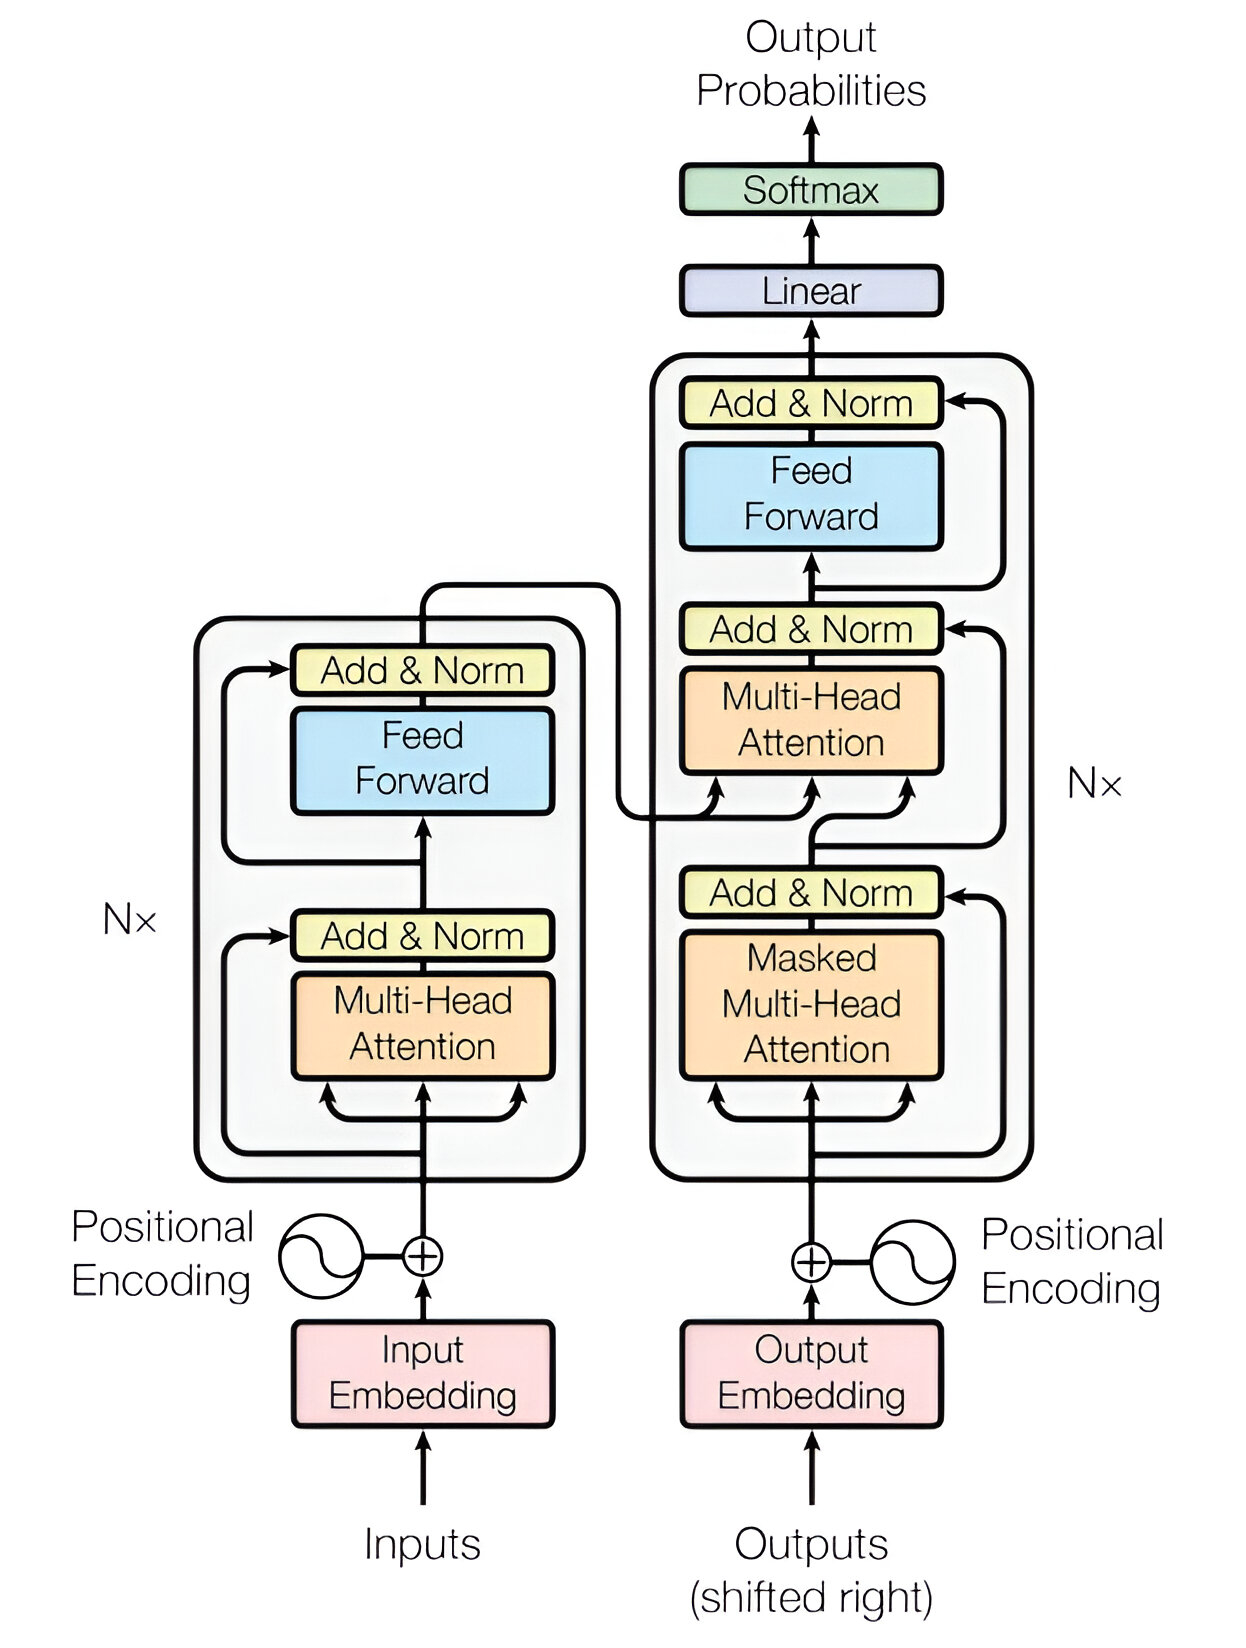
\includegraphics[width=0.7\linewidth]{imagens/transformers-melhor.jpg}
     \label{fig:2}
     \caption*{\textbf{Fonte:} \citeonline{vaswani2017}}
\end{figure}

A arquitetura do Transformer é composta por duas redes neurais principais: o codificador (\textit{encoder}) e o decodificador (\textit{decoder}). Como ilustrado na Figura \ref{fig:2}, cada uma dessas redes é estruturada em múltiplas camadas idênticas empilhadas, onde:

\begin{itemize}
    \item \textbf{Codificador:} Recebe a sequência de entrada, aplica \textit{embeddings} e incorpora informações posicionais. Cada camada contém um bloco de \textit{multi-head self-attention}, seguido por uma camada \textit{feed-forward}. O mecanismo de normalização residual (\textit{Add \& Norm}) mantém a estabilidade do treinamento.
    \item \textbf{Decodificador:} Similar ao codificador, mas incorpora uma camada adicional de \textit{Masked Multi-Head Attention}, que impede o modelo de olhar para \textit{tokens} futuros durante a geração de texto. Após essa etapa, as informações passam pelo mecanismo de atenção cruzada (\textit{cross-attention}), que permite ao decodificador utilizar os estados do codificador para refinar a saída.
\end{itemize}

Na última camada do decodificador, os vetores de saída são projetados para probabilidades através de uma camada linear e \textit{softmax}, que gera a predição final da sequência.

A principal inovação do Transformer está no uso da \textit{Multi-Head Attention}, que permite que diferentes partes da entrada sejam analisadas simultaneamente sob diversas perspectivas. Essa abordagem permite que os modelos lidem com sequências de texto de maneira mais eficiente e paralela, superando limitações anteriores encontradas em redes recorrentes. Sendo assim, a arquitetura Transformers foi um marco para o campo de IA, tornando-se a base para os modelos de LLM mais avançados.

De acordo com \citeonline{devlin2018} e \citeonline{thoppilan2022}, modelos como o GPT (Generative Pre-trained Transformer), BERT (Bidirectional Encoder Representations from Transformers) e LaMDA (Language Model for Dialogue Applications) impulsionaram avanços significativos em diversas tarefas de NLP (Natural Language Processing), como geração de texto, tradução automática, resumo automático e resposta a perguntas. O modelo BERT, por exemplo, introduziu uma abordagem bidirecional que melhora a compreensão contextual das palavras em um texto, enquanto o GPT demonstrou avanços notáveis na geração de texto fluente e coerente. O modelo LaMDA, por sua vez, foi projetado para diálogos naturais, possibilitando interações mais humanizadas e relevantes. Esses avanços mostram o impacto dos LLMs na automação de tarefas cognitivas complexas, oferecendo soluções inovadoras para aplicações comerciais, educacionais e de acessibilidade.

\subsection{LLMs Multimodais}

Os modelos de LLM Multimodais, ou MLLM (Multimodal Large Language Model) são uma evolução significativa dos modelos de linguagem, projetados para processar e gerar informações a partir de diferentes tipos de dados, como texto, imagens e áudio. Da mesma forma que destacado por \citeonline{bala2024}, também é notável a importância destes avanços pelo trabalho de \citeonline{wu2023}:

\begin{citacao}
    O nosso mundo é inerentemente multimodal e os seres humanos percepcionam o mundo com diferentes órgãos sensoriais para informação modal variada, como a linguagem, as imagens, os vídeos e os sons, que muitas vezes se complementam e sinergizam entre si. Com esta intuição, os LLM puramente baseados em texto foram recentemente dotados de outras capacidades de compreensão e de percepção de imagem, vídeo, áudio, etc.
\end{citacao}

Desta forma, modelos como o CLIP, citado no trabalho de \citeonline{radford2021}, demonstram a capacidade de conectar imagens e texto de forma eficaz, aprendendo a representar ambos em um espaço vetorial compartilhado. Essa capacidade permite ao CLIP realizar tarefas como  \textit{zero-shot image classification}, geração de legendas para imagens e  busca de imagens a partir de descrições textuais.

O CLIP é um dos exemplos de modelos que existem com a capacidade multimodal, mas existem vários outros, como o NExT-GPT \cite{wu2023} e o LLaVA \cite{liu2023}. A extensão de modelos MLLM nos últimos anos vem crescendo exponencialmente, como pode-se notar na Figura \ref{fig:3}, elaborada por \citeonline{Yin2024}, evidenciando uma linha do tempo dos MLLMs.

\begin{figure}[!h]
     \caption{Evolução dos Modelos MLLMs}
     \centering
     \includegraphics[width=0.95\linewidth]{imagens/avanços-llms.png}
     \label{fig:3}
     \caption*{\textbf{Fonte:} \citeonline{Yin2024}}
\end{figure}

Em suma, os MLLMs representam uma inovação significativa no campo da inteligência artificial, proporcionando uma compreensão mais abrangente dos dados por meio da integração de múltiplas modalidades. Por fim, fica claro que a gama de modelos possíveis para a utilização é alta, viabilizando diversas aplicações inovadoras que envolvem vários tipos de entrada, voltadas para acessibilidade, automações e outras áreas equivalentes.

\subsection{LLMs e MLLMs \textit{Open Source}}

Os LLMs e MLLMs de código aberto oferecem vantagens significativas para pesquisadores, desenvolvedores e organizações que buscam soluções avançadas em inteligência artificial. Uma plataforma central nesse ecossistema é a Hugging Face, que se destaca como um repositório líder para modelos de código aberto.

\begin{citacao}
    Hugging Face (HF) e seu Hub se destacam nesse aspecto [pesquisa e desenvolvimento de IA] devido ao seu papel crítico no desenvolvimento, compartilhamento e implantação de uma ampla gama de modelos de ML, incluindo Large Language Models (LLMs) e IA generativa. \cite{Castano2023}
\end{citacao}

\subsubsection{Hugging Face}

Valendo-se da própria definição existente na página da empresa Hugging Face:

\begin{citacao}
    O Hugging Face Hub é uma plataforma com mais de 900 mil modelos, 200 mil conjuntos de dados e 300 mil demonstrações nas quais as pessoas podem colaborar facilmente em seus fluxos de trabalho de ML. O Hub funciona como um local central onde qualquer pessoa pode compartilhar, explorar, descobrir e experimentar o Machine Learning de código aberto. \cite{huggingface2023}
\end{citacao}

Desta forma, é nítido que o Hugging Face mostra-se como uma fonte confiável e valiosa na busca de bons modelos de LLMs, proporcionando uma infraestrutura robusta para pesquisadores, desenvolvedores e empresas que desejam explorar e implementar soluções de inteligência artificial de forma eficiente e colaborativa. A ampla variedade de modelos disponíveis, abrangendo diferentes arquiteturas e domínios de aplicação, permite que usuários encontrem soluções adequadas às suas necessidades específicas, reduzindo o tempo e os custos associados ao desenvolvimento de modelos do zero.

Assim, o Hugging Face não apenas democratiza o acesso à inteligência artificial de ponta, mas também fomenta um ecossistema aberto e dinâmico, onde inovação e conhecimento são compartilhados globalmente, impulsionando o avanço contínuo da área de aprendizado de máquina.

\subsection{Métricas de Avaliação}

A avaliação da qualidade das descrições geradas por LLMs é um aspecto fundamental para garantir a precisão e a relevância das informações fornecidas. Tradicionalmente, métricas como BLEU \cite{Papineni2001}, METEOR \cite{banerjee2005} e CIDEr \cite{Vedantam2015} têm sido amplamente utilizadas para comparar as legendas geradas com referências humanas, analisando a similaridade baseada em n-gramas e a estrutura das sentenças. Embora essas métricas ofereçam uma avaliação quantitativa eficaz, elas podem não capturar adequadamente aspectos semânticos e contextuais mais complexos das descrições.

Nesse sentido, métricas mais recentes, como CLIPScore \cite{hessel-etal-2021-clipscore}, VQAScore \cite{lin2024} e o BERTScore \cite{Zhang2020:}, têm sido introduzidas para fornecer uma avaliação mais abrangente. Essas métricas utilizam modelos avançados de aprendizado profundo para medir a similaridade semântica entre a imagem e a legenda gerada, levando em consideração o alinhamento contextual e o significado subjacente ao conteúdo visual.

Assim, a utilização de métricas tradicionais e/ou modernas permite uma análise mais robusta da qualidade das descrições, equilibrando aspectos quantitativos e qualitativos. O uso dessas abordagens contribui para uma avaliação mais fiel à experiência humana, impulsionando o desenvolvimento de sistemas de IA cada vez mais eficazes e coerentes na interpretação e descrição de conteúdos visuais.

\section{Processamento de Voz: \textit{Speech-to-Text} (STT) e \textit{Text-to-Speech} (TTS)}

As tecnologias de Processamento de Voz permitem a interação entre humanos e computadores por meio da linguagem falada, possibilitando a conversão entre voz e texto. Esta seção explora duas tecnologias chave neste domínio: \textit{Speech-to-Text} (STT) e \textit{Text-to-Speech} (TTS), com foco em seus conceitos,  funcionamento e aplicações, especialmente em acessibilidade.

\subsection{Reconhecimento de Voz: \textit{Speech-to-Text}}

O Reconhecimento de Voz, conhecido como \textit{Speech-to-Text} ou Reconhecimento Automático de Voz (ASR, do inglês Automatic Speech Recognition), é uma tecnologia que converte a linguagem falada em texto escrito. Segundo \citeonline{Alharbi2021}, o ASR começou com sistemas simples que respondiam a um número limitado de sons e evoluiu para sistemas sofisticados que respondem fluentemente à linguagem natural, desta forma, facilitando a comunicação entre humanos e máquinas.

O processo de conversão da fala em texto, embora pareça simples,  envolve uma série de etapas complexas. De acordo com Trivedi et al. (2018), a arquitetura de um sistema STT segue as seguintes etapas:

\begin{itemize}
    \item \textbf{Pré-processamento:} O sinal de fala analógico é convertido em formato digital para processamento posterior. Técnicas de remoção de ruído e normalização são aplicadas para melhorar a qualidade do áudio;
    \item \textbf{Feature Extraction:} Técnicas como os Coeficientes Cepstrais de Frequência Mel (MFCC) e Linear Predictive Coding (LPC) são utilizadas para extrair características relevantes da fala, fornecendo uma representação compacta do áudio. Essas características servem de base para a modelagem acústica subsequente;
    \item \textbf{Modelagem Acústica:} Responsável por correlacionar os sinais acústicos aos fonemas da língua. Modelos como os Modelos Ocultos de Markov (HMMs) e redes neurais profundas (DNNs) são amplamente utilizados nessa fase.
    \item \textbf{Modelagem de Linguagem:} Prediz a sequência mais provável de palavras com base em regras linguísticas e dados estatísticos. Auxilia na redução de ambiguidades e melhora a precisão da transcrição.
    \item \textbf{Decodificação:} Integra informações dos modelos acústico e de linguagem para gerar a transcrição mais precisa. Algoritmos de busca, como o Viterbi, são frequentemente utilizados nesta fase.
\end{itemize}

A Figura \ref{fig:4} apresenta a arquitetura geral de um sistema de reconhecimento de fala conforme descrito no artigo de \citeonline{trivedi2018}:

\begin{figure}[!h]
     \caption{Exemplo Arquitetura STT}
     \centering
     \includegraphics[width=0.7\linewidth]{imagens/stt.png}
     \label{fig:4}
     \caption*{\textbf{Fonte:} \citeonline{trivedi2018}}
\end{figure}

Alguns modelos que podem ser usados incluem o Whisper, da OpenAI \cite{radford2023}, e outros como o próprio Google Cloud Speech-to-Text e o wav2vec 2.0 \cite{Baevski2020}.

\subsection{Síntese de Voz: \textit{Text-to-Speech}}

A Síntese de Voz, conhecida como \textit{Text-to-Speech} (TTS), é uma tecnologia que converte texto escrito em fala artificial, permitindo que sistemas computacionais transformem conteúdos de texto em áudio. Segundo \citeonline{trivedi2018}, essa tecnologia tem sido amplamente utilizada em diversas aplicações, como assistentes virtuais, leitores de tela para acessibilidade e sistemas de navegação. O objetivo do TTS é transformar texto em um áudio inteligível e natural, aproximando-se ao máximo da fala humana.

O fluxo realizado pelas aplicações que realizam a síntese de voz possui basicamente dois módulos principais. De acordo com \citeonline{Dutoit1997}, são eles o módulo de Processamento de Linguagem Natural (NLP, do inglês Natural Language Processing) e o módulo de Processamento de Sinal Digital (DSP, do inglês Digital Signal Processing). \citeonline{Dutoit1997} explica que, de forma bem parecida com a fala humana:

\begin{citacao}
    …ela compreende um módulo de Processamento de Linguagem Natural (NLP), capaz de produzir uma transcrição fonética do texto lido, juntamente com a entonação e o ritmo desejados (frequentemente denominado como prosódia), e um módulo de Processamento de Sinal Digital (DSP), que transforma a informação simbólica que recebe em fala.
\end{citacao}

Na Figura \ref{fig:5}, pode-se perceber mais facilmente como o diagrama do sistema TTS processa as informações, primeiramente com um módulo de NLP, transcrevendo foneticamente o texto lido e, posteriormente, o texto é submetido ao módulo de DSP, que realiza a transformação do texto em fala.

\begin{figure}[!h]
     \caption{Exemplo simples do funcionamento do TTS}
     \centering
     \includegraphics[width=0.7\linewidth]{imagens/tts.png}
     \label{fig:5}
     \caption*{\textbf{Fonte:} \citeonline{Dutoit1997}}
\end{figure}

Assim, embora a estrutura tradicional de sistemas TTS, baseada nos módulos de NLP e DSP, ainda seja amplamente utilizada, modelos mais modernos adotam arquiteturas aprimoradas para superar limitações de desempenho e qualidade da fala. Segundo \citeonline{popov2021}, as abordagens atuais incorporam técnicas de modelagem difusional probabilística, como o modelo Grad-TTS, que emprega um decodificador baseado em score para transformar gradualmente o ruído em mel-espectrogramas alinhados ao texto de entrada, utilizando o algoritmo de Monotonic Alignment Search (MAS) para aprimorar a correspondência entre texto e áudio. Essa abordagem permite um controle explícito do equilíbrio entre qualidade da síntese e velocidade de inferência, representando um avanço significativo sobre os métodos tradicionais baseados em atenção, como o Tacotron2.

Dessa forma, os sistemas modernos de TTS evoluíram para incorporar arquiteturas mais robustas, capazes de fornecer fala sintetizada com maior naturalidade e precisão, ao mesmo tempo em que reduzem os erros de pronúncia e aumentam a eficiência computacional.